
\begin{frame}{Un paso do procesador}
  \begin{columns}[c]
    \begin{column}{0.36\textwidth}
      \small
      \begin{itemize}
        \item Primeiro \destacado{aténdese ás interrupcións} pendentes segundo a súa prioridade.
        \item Se non as hai, búscase, decodifícase e execútase a instrución.
        \item O tempo consumido é o que despois fai avanzar
          \textsc{ppu}, \textsc{apu}, temporizadores e porto serie.
      \end{itemize}
    \end{column}
    \begin{column}{0.62\textwidth}
      \begin{center}

        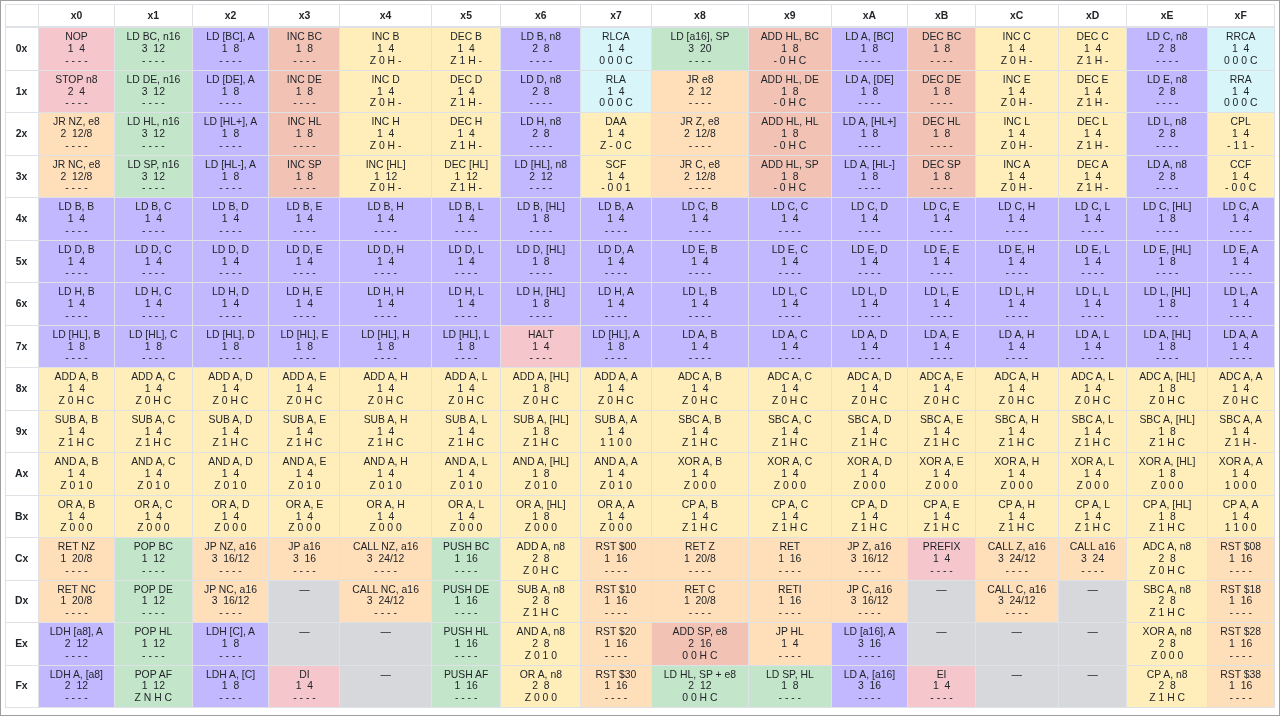
\includegraphics[width=\textwidth,height=0.74\textheight,keepaspectratio]{imaxes/sm83_instruction_set.png}\\[0.3em]
        \fonte{Táboa principal de \textit{opcodes}.}

      \end{center}
    \end{column}
  \end{columns}
\end{frame}

\begin{frame}{Execución dunha instrución}
  \vfill
  \begin{itemize}
    \setlength{\itemsep}{1.1em}
    \item Unha instrución é un \texttt{struct} que implementa
      \texttt{Instruction} e o operando é un \destacado{parámetro xenérico}
      que xa sabe o seu tamaño e o seu custo en ciclos.
    \item \texttt{exec} le o operando fonte, escribe no destino e devolve o
      efecto da instrución.
    \item \texttt{InstructionEffect} devolve o tempo consumido e as
      bandeiras: cada unha pode quedar a \texttt{true}, a \texttt{false} ou
      \destacado{sen cambios}.
    \item \texttt{info} resólvese a partir das constantes asociadas dos
      operandos, \destacado{en tempo de compilación}.
    \item Un módulo por instrución, sen código repetido e sen custo
      en tempo de execución.
  \end{itemize}
  \vfill
\end{frame}

\begin{frame}[fragile]{Execución dunha instrución}
\begin{lstlisting}[language=Rust,basicstyle=\ttfamily\fontsize{7.8pt}{8.3pt}\selectfont,breaklines=false]
pub struct Ld<D: WritableOperand, S: Operand> {
  dst: D,
  src: S,
}
impl<D: WritableOperand, S: Operand> Ld<D, S> {
  pub fn new(dst: D, src: S) -> Self { Self { dst, src } }
}
impl<D: WritableOperand, S: Operand> Instruction for Ld<D, S> {
  fn exec(&mut self, gb: &mut Dmg) -> InstructionResult {
    let value = self.src.read(gb);
    self.dst.write(gb, value);

    Ok(InstructionEffect::new(self.info(), Flags::none()))
  }
  fn info(&self) -> (u8, u8) {
    (1 + S::READ_CYCLES + D::WRITE_CYCLES, 1 + S::LEN + D::LEN)
  }
  fn disassembly(&self) -> String {
    format!("ld {},{}", self.dst, self.src)
  }
}
\end{lstlisting}
\end{frame}



\begin{frame}{Unidade de procesamento de píxeles}
  \begin{columns}[c]
    \begin{column}{0.44\textwidth}
      \small
      \begin{itemize}
        \item Unha máquina de estados percorre os modos da \textsc{ppu}:
        \texttt{OAM search}, \texttt{pixel transfer}, \texttt{HBlank} e \texttt{VBlank}.
        
        \item \textit{scanline rendering} debuxa cada liña con \texttt{draw\_bg}, \texttt{draw\_window} e \texttt{draw\_sprites},
        de esquerda a dereita resolvendo prioridades e transparencia.
        
        \item O fondo garda unha \destacado{caché de identificadores de cor}
        coa que despois se resolven as prioridades dos obxectos facilmente.

      \end{itemize}
    \end{column}
    \begin{column}{0.54\textwidth}
      \imaxe[\textwidth]{imaxes/ppu_composition.png}{Composición dun cadro: fondo, xanela e obxectos.}
    \end{column}
  \end{columns}
\end{frame}


\begin{frame}[plain,noframenumbering]
  \begin{center}
    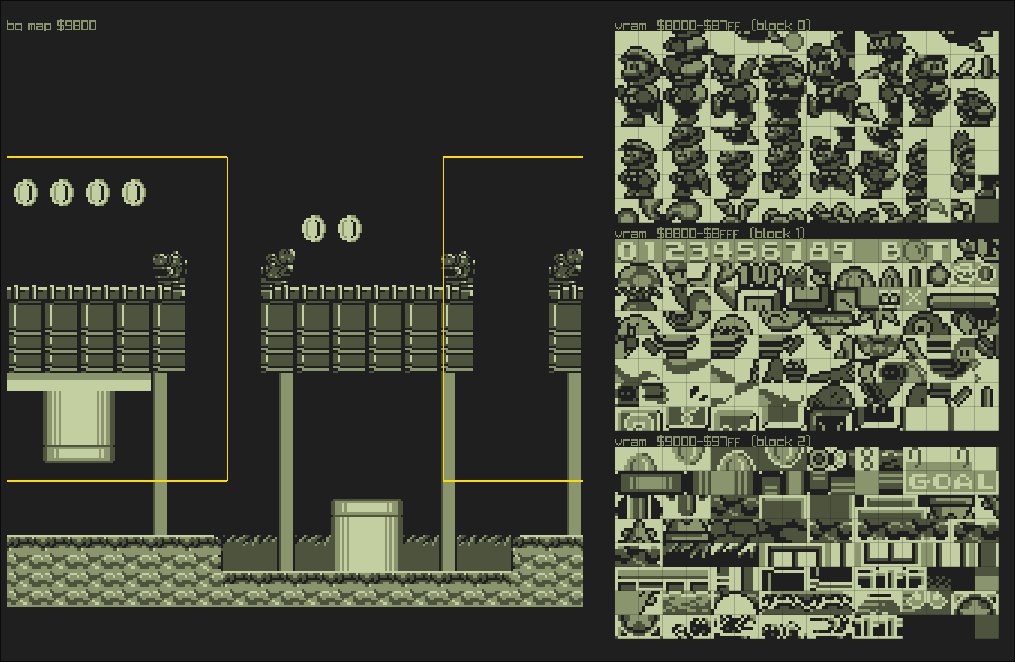
\includegraphics[width=0.84\textwidth,height=0.76\textheight,keepaspectratio]{imaxes/vram_oam_representation.png}\\[0.4em]
    \fonte{Ferramentas de depuración: contido da \textsc{vram} e dos obxectos da \textsc{oam}.}
  \end{center}
\end{frame}

\begin{frame}{Os cartuchos amplían o hardware da consola}
  \vfill
  \begin{itemize}
    \setlength{\itemsep}{1.4em}

    \item A Game Boy emprega os cartuchos para engadir hardware adicional
    A configuración deste hardware faise mediante escrituras no espazo de direccións da \textsc{rom}.

    \item O \textsc{mbc} encárgase de xestionar ese hardware. Existen moitos,
    dos que se implementaron os cinco máis habituais: sen \textsc{mbc},
    \textsc{mbc}1, \textsc{mbc}2, \textsc{mbc}3 e \textsc{mbc}5.

    \item O seu cometido principal é \destacado{intercambiar os bancos de
    \textsc{rom} e \textsc{ram}} para aumentar a memoria dispoñible.

  \end{itemize}
  \vfill
\end{frame}

\begin{frame}[fragile]{Os cartuchos amplían o hardware da consola}
\begin{lstlisting}[language=Rust,breaklines=false]
fn write_rom(&mut self, address: u16, value: u8) {
  match address {
    RAM_AND_TIMER_ENABLE_START..=RAM_AND_TIMER_ENABLE_END => {
      let enabled = (value & 0x0F) == 0x0A;
      ...
    }

    ROM_BANK_NUMBER_START..=ROM_BANK_NUMBER_END => {
      self.rom_selected_bank = value & 0x7F;
    }

    RAM_BANK_NUMBER_OR_RTC_SELECT_START..=RAM_BANK_NUMBER_OR_RTC_SELECT_END => {
      if value <= 0x03 {
        self.ram_selected_bank = value;
        self.rtc_selected = false;
        ...
\end{lstlisting}
\end{frame}

\begin{frame}{Optimización}
  \begin{columns}[c]
    \begin{column}{0.46\textwidth}
      \small
      \begin{itemize}
        \item \destacado{Bucles de debuxado}: reutilizar cálculos entre píxeles
        consecutivos e acceso directo ás memorias da \textsc{ppu}.

        \item \destacado{Complexidade}: temporizador e \textsc{apu} son
        contadores periódicos; en vez de iterar nun bucle segundo o tempo avanzado pola \textsc{cpu},
        % calculase canto tempo falta para o seguinte evento e avánzase directamente.

        \item \destacado{Bucle quente}: elimminouse o uso de memoria no \textit{heap} no bucle quente
        e o \textit{dynamic dispatching} substituíuse por resolución estática e monomorfización.
      \end{itemize}
    \end{column}
    \begin{column}{0.52\textwidth}
      \begin{center}
        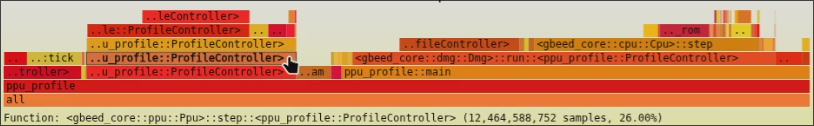
\includegraphics[width=\textwidth]{imaxes/flamegraph_baseline.png}\\[0.2em]
        \fonte{Antes: o debuxado supón o 26,0\,\% do tempo.}\\[0.7em]
        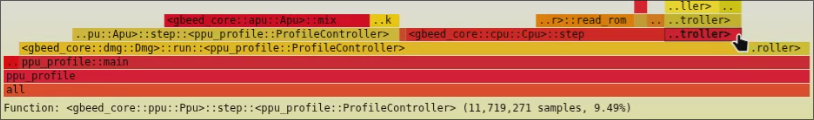
\includegraphics[width=\textwidth]{imaxes/flamegraph_optimized.png}\\[0.2em]
        \fonte{Despois: 9,5\,\%.}
      \end{center}
    \end{column}
  \end{columns}
\end{frame}

\begin{frame}{Dúas interfaces sobre o mesmo núcleo}
  \vfill
  \begin{block}{Interface de depuración}
    Amosa o estado da \textsc{vram} e a entrada do mando. % moi util para comprobar erro
    Compilada a WebAssembly con Emscripten e despregada en GitHub Pages
    con cada confirmación.
  \end{block}
  \vspace{1em}
  \begin{block}{Interface de estilo consola}
    Consegue unha experiencia de usuario similar á unha consola.
    Incorpora menús para o control do emulador e varias características de calidade de vida
  \end{block}
  \vfill
\end{frame}

\begin{frame}{Do emulador á consola}
  \begin{columns}[c]
    \begin{column}{0.46\textwidth}
      \small
      \begin{itemize}

        \item \destacado{Raspberry Pi Zero W} (\texttt{armv6l}) e
        \destacado{Zero 2 W} (\texttt{aarch64}).

        \item \destacado{GamePi13}: pantalla \textsc{IPS} con controlador
        ST7789, altofalante e botóns, conectado aos \textsc{gpio} \textbf{sen soldadura}.

      \end{itemize}
    \end{column}
    \begin{column}{0.52\textwidth}
      \imaxe[\textwidth]{imaxes/gamepi13.png}{A construción de referencia executando o emulador.}
    \end{column}
  \end{columns}
\end{frame}

\begin{frame}{Unha imaxe de sistema reproducible}
  \footnotesize
  \begin{columns}[t]
    \begin{column}{0.49\textwidth}
      \begin{block}{NixOS en RPi Zero 2 W}
        \begin{itemize}
          \item A pantalla emprégase co controlador \texttt{panel-mipi-dbi},
          en vez de usar o \textit{stack} obsoleto documentado polo fabricante.

          \item O \textit{firmware} de inicialización do ST7789V e o
          \textit{overlay} do audio por \textsc{pwm} xéranse en tempo de evaluación,
          sen configuración manual requerida.

          \item Emprégase o núcleo \texttt{drm} de Raylib sen unha sesión gráfica completa. 

          \item Unha imaxe de \textsc{sd} lista para gravar que arranca o emulador directamente,

        \end{itemize}
      \end{block}
    \end{column}
    \begin{column}{0.49\textwidth}
      \begin{block}{Debian do fabricante en RPi Zero W}
        \begin{itemize}
          \item \texttt{armv6l} non está soportada por NixOS polo que o mellor é partir da imaxe preconfigurada do fabricante.

          \item \textit{fbcp} copia o \textit{framebuffer} principal a través de DispmanX
          e só funciona sobre X11.

          \item \destacado{Materializouse un dos riscos previstos}. Obrigou a
          cambiar o backend \textsc{drm} polo de X11.

          \item O binario obtense por compilación cruzada nun contedor.
        \end{itemize}
      \end{block}
    \end{column}
  \end{columns}
\end{frame}

\begin{frame}[fragile]{Unha imaxe de sistema reproducible}
\begin{lstlisting}[language=Nix,breaklines=false]
{
  inputs,
  outputs,
  ...
}: {
  gbeed02 = inputs.nixpkgs-pi.lib.nixosSystem {
    specialArgs = {
      inherit inputs outputs;
      hostname = "gbeed02";
      username = "gbeed";
    };
    modules = [
      "${inputs.nixpkgs-pi}/nixos/modules/installer/sd-card/sd-image-aarch64.nix"
      ./gbeed02/configuration.nix
      ./gbeed02/hardware-configuration.nix
    ];
  };
}
\end{lstlisting}
\end{frame}
